\section{Implementation}
This section will discuss the implementation of each module and the way they integrate together to make the computer. Figure \ref{fig:computer} shows the computer as it was in January 25, which was its first working state. In Figure \ref{fig:computer_parts} the overlays show where each of the modules are located.

\begin{figure}[H]
  \centering
  % TODO: high resulotion version
  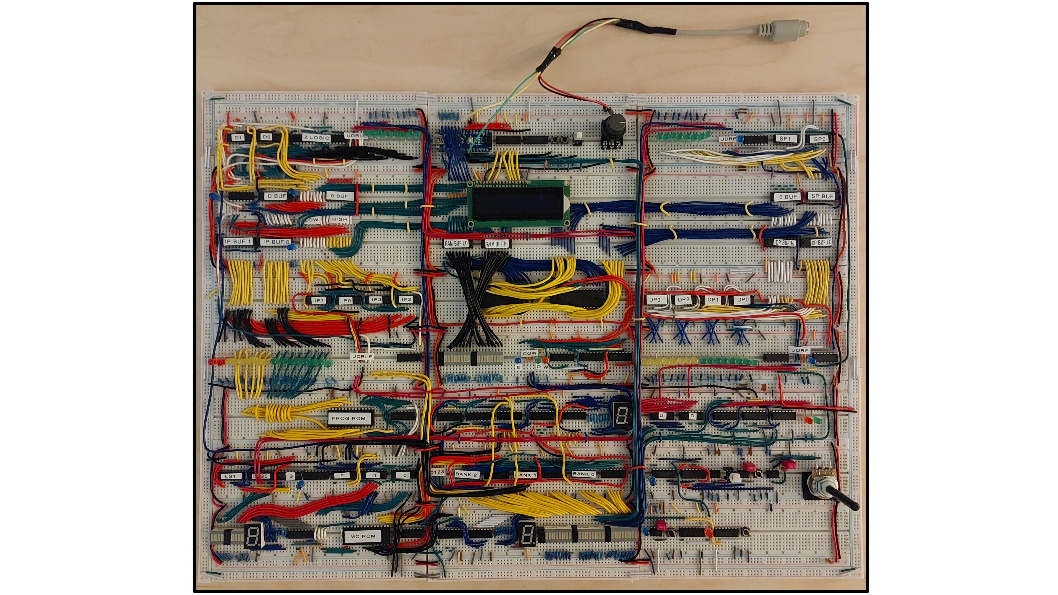
\includegraphics[width=0.9\textwidth]{img/computer}
  \caption{Prototype in January 2025.}
  \label{fig:computer}
\end{figure}

\begin{figure}[H]
  \centering
  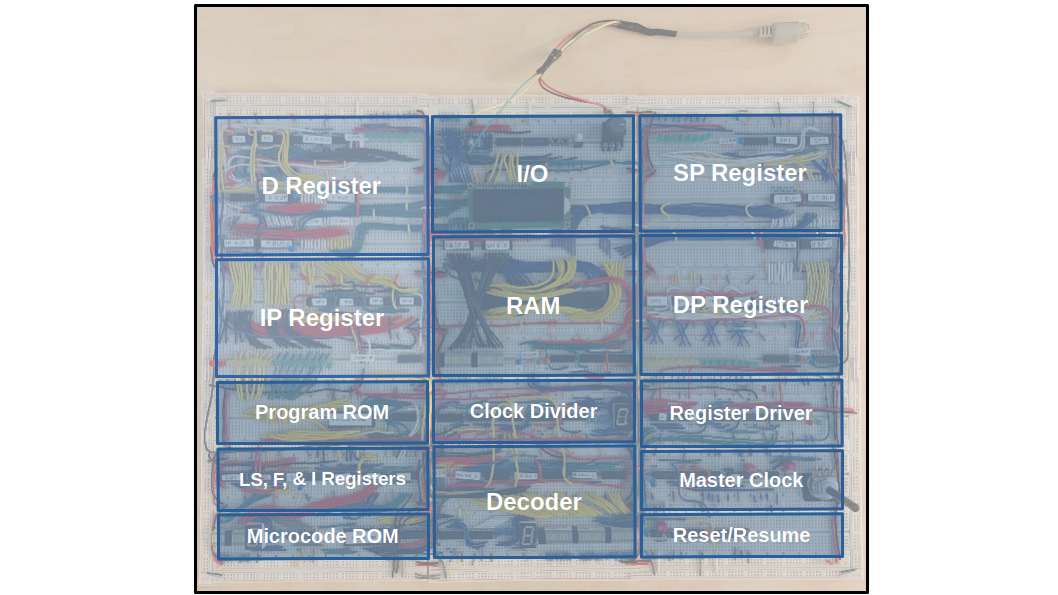
\includegraphics[width=0.9\textwidth]{img/computer_parts}
  \caption{Overview of the different parts of the computer.}
  \label{fig:computer_parts}
\end{figure}

\subsection{Master Clock and Reset/Resume}
The Master Clock module (MC) is located at the bottom right of the computer and is responsible for providing a heartbeat to most of the modules. The design of the clock is taken directly from Ben Eater's 8-bit computer video's \cite{beneater}. The reason this module is called \emph{Master} Clock (rather than just Clock) is that the output of this module is not serving directly as the clock to all of the modules. For reasons becoming apparent when the implementation of the decoding process is discussed (see \ref{sec:implementation:clockdivider}), this clock is divided into 4 subclock-pulses, the last of which is sent to the modules. Effectively,  the frequency at which the computer operates is only one fourth that of the output from the MC.

The Reset/Resume module is directly underneath the clock and contains some logic to be able to reset the computer (necessary after applying power) and resuming the clock when it is halted. The HLT signal coming from the decoder is latched into a register (74LS173) from which the corresponding output bit is connected to the HLT input of the Master Clock selection logic. When the system is reset using the reset button or when the resume button is pressed, the HLT bit is cleared and the clock resumes. This allows for pausing and resuming the computer, effectively adding breakpoints in the code. The reset button itself is debounced in the same way as the manual clock button to ensure a stable transition. 

\subsubsection{Stability}
When the output of the clock was first connected a counting register within the clock divider, it turned out that its output signal was too noisy for reliable operation of the counter. This register (74LS161) is sensitive to even very short pulses and the logic responsible for selecting either the automatic clock or the manual pulses was adding too much noise. The selection logic was modified to use a Schmitt Trigger (74LS14) at its output (rather than a regular inverter like the 74LS04) to improve output signal quality. A Schmitt Trigger acts as an inverter with different thresholds for each direction of inversion. This means it will invert any incoming signal above some voltage threshold but when the input goes below that same threshold shortly after due to noise, it will not change its output again until the signal drops significantly. Once the Schmitt Trigger was implemented, all stability issues went away.

\subsubsection*{Parts}
\begin{itemize}\itemsep0em
\item 4x NE555P (555 Timer)
\item 1x 74LS14 (Schmitt Trigger Inverter)
\item 1x 74LS00 (NAND)
\item 1x 74LS173 (4 bit register)
\item 1x 74LS32 (OR)
\item 4x $0.01\mu F$ ceramic capacitor
\item 3x $1\mu F$ capacitor
\item 3x tactile switch
\item 1x latching push button
\item 1x potentiometer (0-1M)
\item 6x 1K resistor
\item 1x 200K resistor
\item 1x 470K resistor
\end{itemize}

\subsubsection*{Schematic}
A full schematic is provided on the next page.
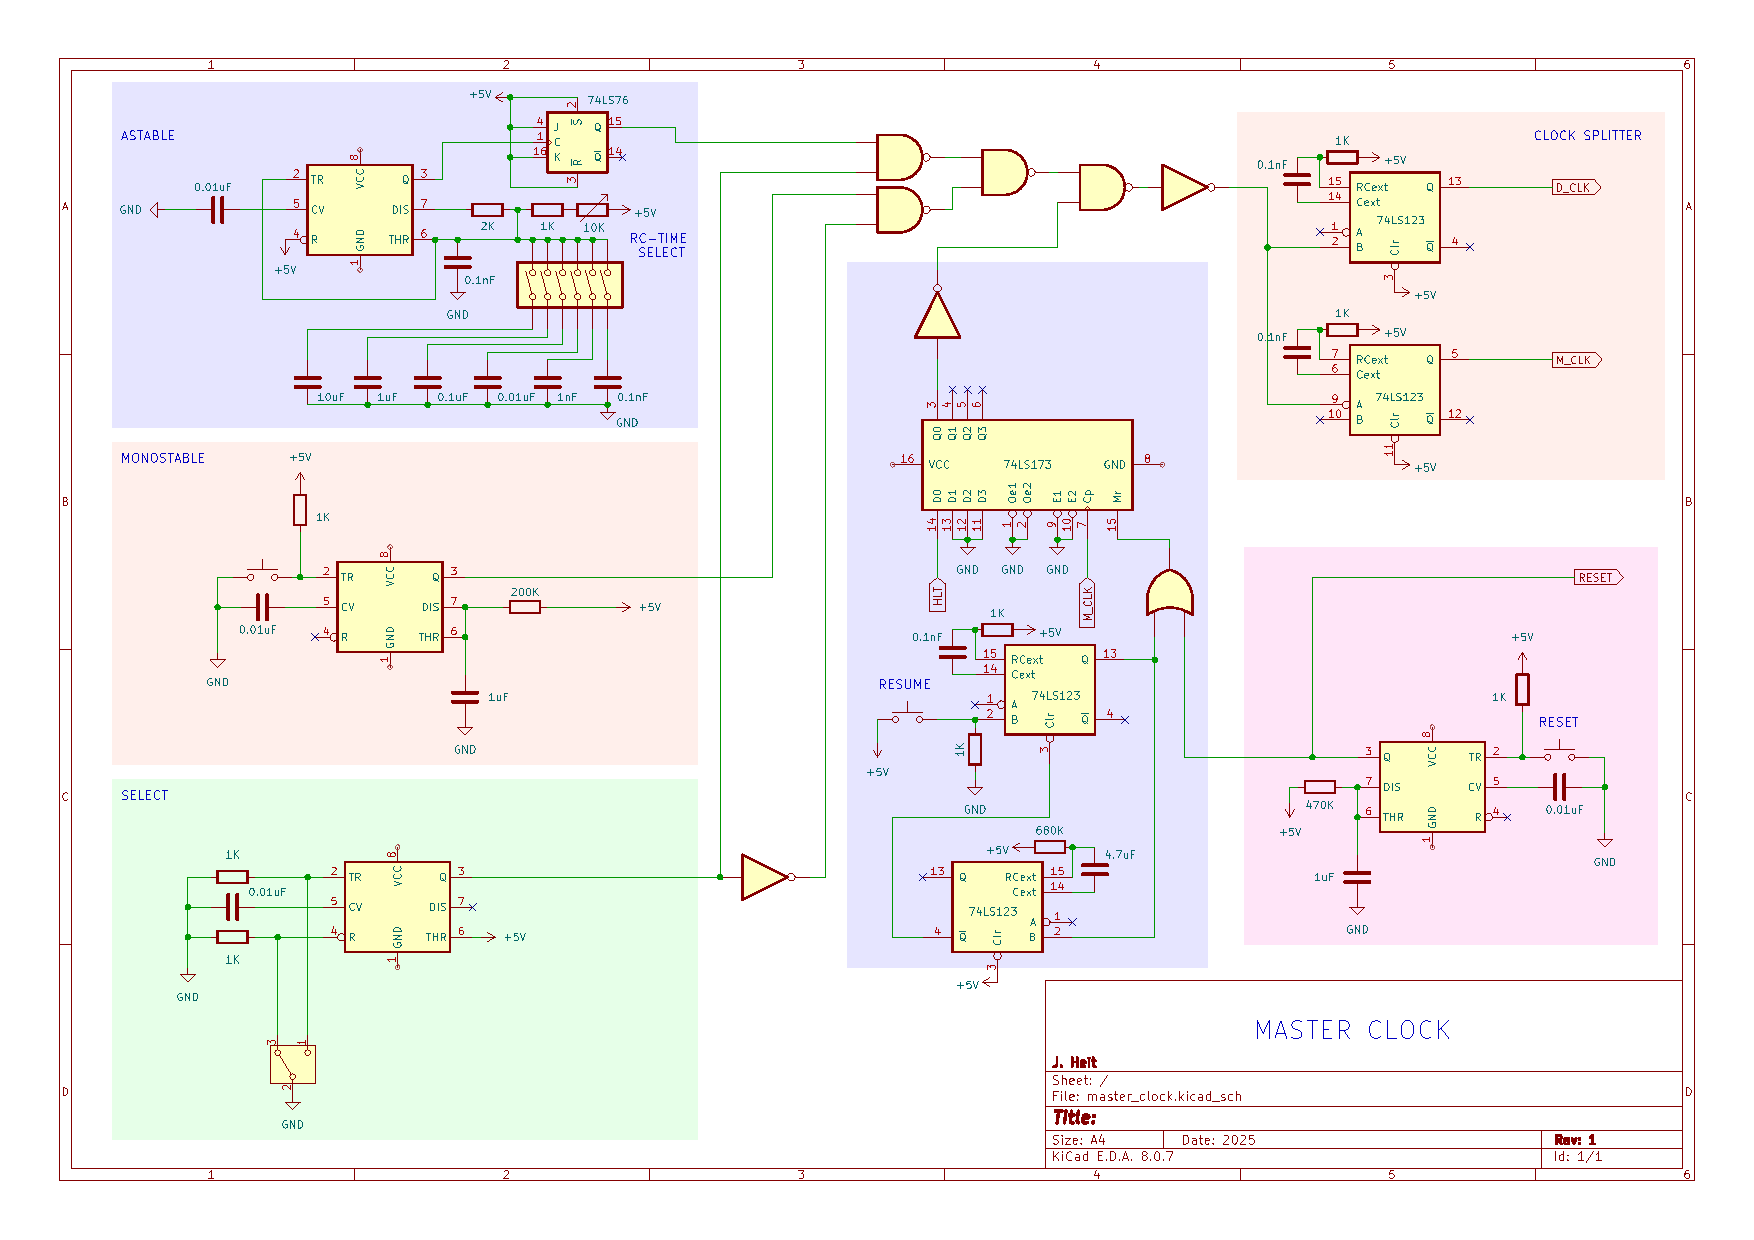
\includepdf[landscape=true]{schematics/masterclock.pdf}

\subsection{Registers}
\subsection{Memory}
\subsection{Control Unit}
\subsection{Screen}
\subsection{Keyboard}
